\documentclass{beamer}
\usetheme{Boadilla}
\usecolortheme{seahorse}
\setbeamertemplate{caption}[numbered]
\usepackage[french,provide=*]{babel}
\usepackage{verbatim}
\usepackage{graphicx}
\usepackage[french,onelanguage]{algorithm2e}
\usepackage{hyperref}

% Personnalisation des couleurs et du style
\definecolor{myblue}{RGB}{0,83,138}
\definecolor{mygray}{RGB}{240,240,240}
\setbeamercolor{frametitle}{bg=myblue,fg=white}
\setbeamercolor{title}{bg=myblue,fg=white}
\setbeamercolor{block title}{bg=myblue!70,fg=white}
\setbeamercolor{block body}{bg=mygray,fg=black}
\setbeamercolor{section in toc}{fg=myblue}

\title[Optimisation IA pour Reversi]{Reversi: Optimisation algorithmique et mémoire}
\author{LAICHE\and GHODBANE\and BAADACHE}

\begin{document}

\begin{frame}
    \titlepage
\end{frame}

\begin{frame}
    \frametitle{Plan de la présentation}
    \tableofcontents
\end{frame}

\section{Introduction et contexte}

\begin{frame}
    \frametitle{Développement incrémental de notre IA}
    
    \begin{block}{Progression méthodique}
    \small
    \begin{itemize}
        \item \textbf{Étapes 1-2} : Implémentation du jeu et IA aléatoire
        \item \textbf{Étape 3} : Arbre de jeu et Minimax (évaluation par différence de pions)
        \item \textbf{Étape 4} : Arbre de jeu (profondeur variable) et détection des ensembles alignés (2 et 3+)
        \item \textbf{Étape 5} : Alpha-beta et une évaluation des positions stratégiques
    \end{itemize}
    \end{block}
    
    \begin{block}{Innovations majeures présentées}
    \small
    \begin{itemize}
        \item \textbf{Optimisation mémoire} : réduction de 98\% de l'empreinte mémoire
        \item \textbf{NegaScout avec tri des coups} : amélioration d'Alpha-Beta
        \item \textbf{Détection d'endgame} : stratégie spécialisée en fin de partie
    \end{itemize}
    \end{block}
\end{frame}

\section{Optimisation mémoire}

\begin{frame}
    \frametitle{Optimisation mémoire : problématique et approche}
    
    \begin{columns}
        \begin{column}{0.48\textwidth}
            \begin{block}{Problématique}
            \scriptsize
            \begin{itemize}
                \item Explosion exponentielle de la mémoire avec la profondeur
                \item Limites pratiques pour explorer au-delà de la profondeur 6
                \item Construction d'arbres complets trop coûteuse en mémoire
            \end{itemize}
            \end{block}
        \end{column}
        \begin{column}{0.48\textwidth}
            \begin{block}{Notre approche innovante}
            \scriptsize
            \begin{itemize}
                \item Un seul \texttt{Plateau} au lieu d'un arbre complet
                \item Structure \texttt{HistoriqueCoup} pour enregistrer les modifications
                \item Application d'un coup puis annulation systématique
                \item Compteurs précis pour suivre la mémoire utilisée
            \end{itemize}
            \end{block}
        \end{column}
    \end{columns}
    
    \begin{block}{Protocole expérimental}
    \scriptsize
    \begin{itemize}
        \item Comparaison de deux approches sur environ 30 plateaux simulant une partie
        \item Mesure de la mémoire utilisée pour différentes profondeurs (1 à 7)
        \item Analyse automatisée des résultats (script Python)
    \end{itemize}
    \end{block}
\end{frame}

\begin{frame}
    \frametitle{Optimisation mémoire : consommation moyenne par coup}
    
    \begin{center}
        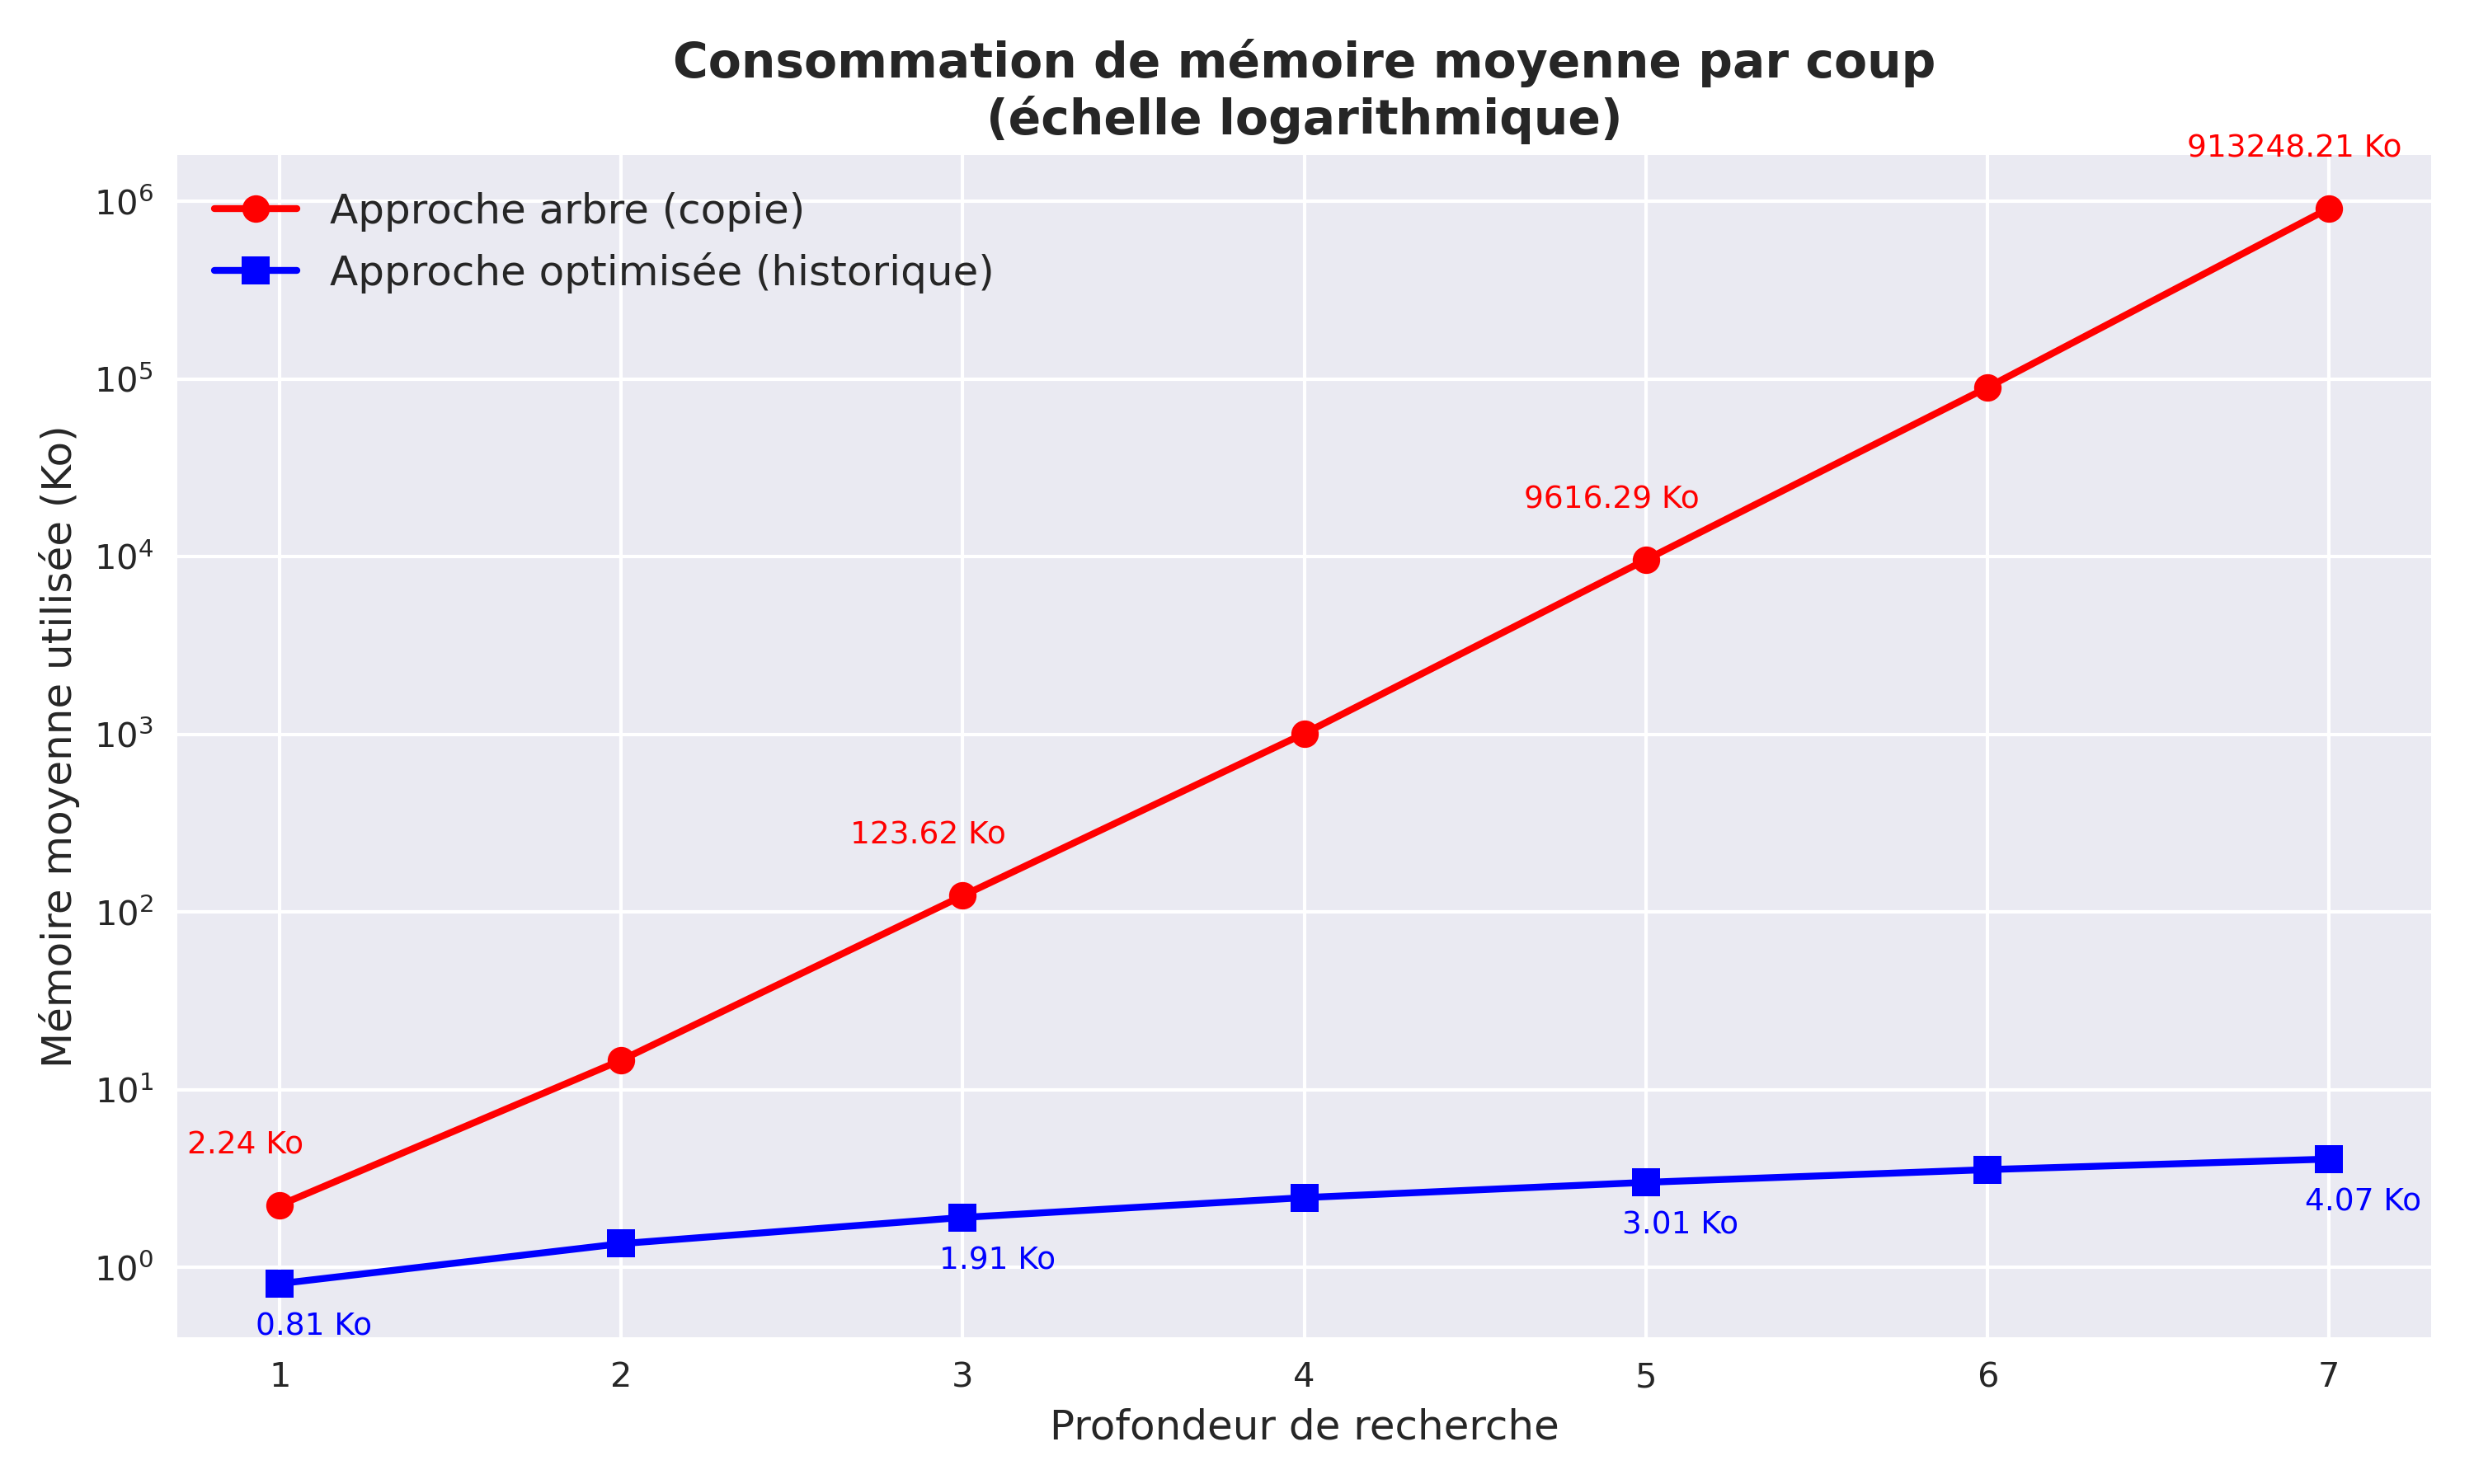
\includegraphics[width=0.7\textwidth]{../assets/memoire_moyenne.png}
    \end{center}
    
    \begin{block}{Analyse des résultats}
    \scriptsize
    \begin{itemize}
        \item \textbf{À profondeur 3} : 123,62 Ko vs 1,91 Ko = réduction de \textbf{98,5\%}
        \item \textbf{À profondeur 5} : 9616,29 Ko vs 3,01 Ko = réduction de \textbf{99,97\%}
        \item \textbf{À profondeur 7} : 913248,21 Ko vs 4,07 Ko = réduction de \textbf{99,99\%}
        \item La différence s'accentue exponentiellement avec la profondeur
    \end{itemize}
    \end{block}
\end{frame}

\begin{frame}
    \frametitle{Optimisation mémoire : impact sur la partie complète}
    
    \begin{center}
        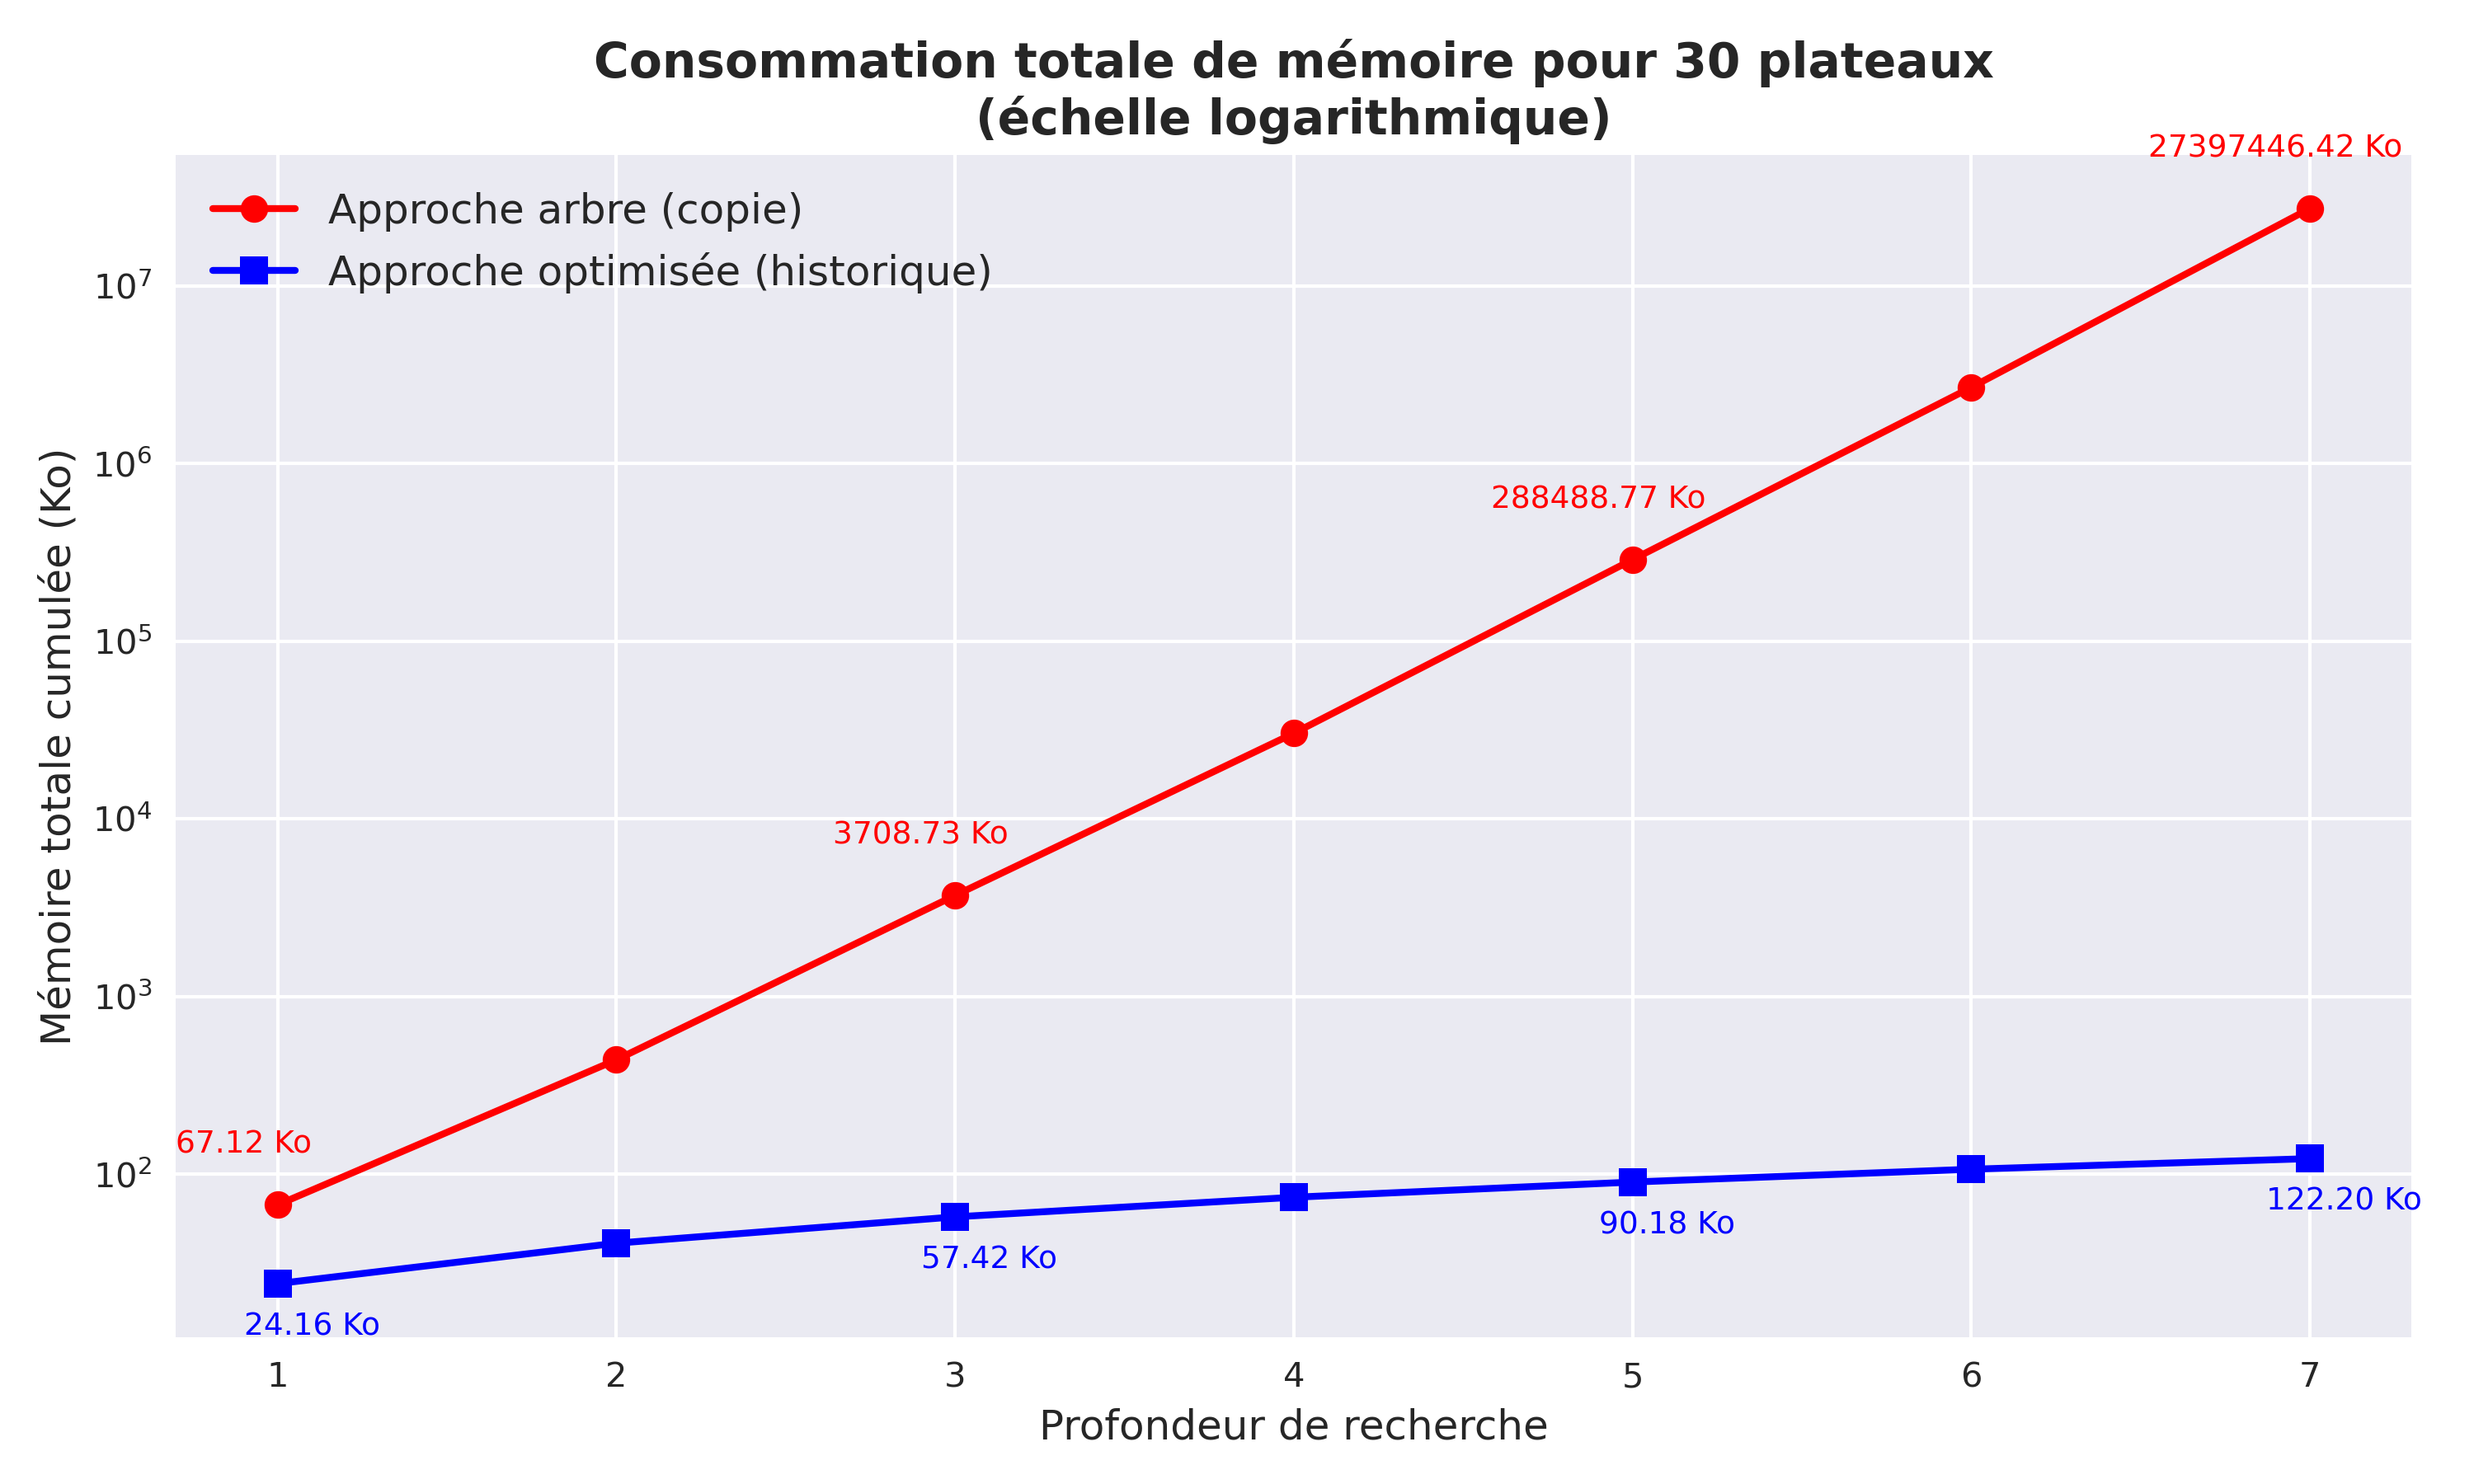
\includegraphics[width=0.7\textwidth]{../assets/memoire_totale.png}
    \end{center}
    
    \begin{block}{Implications pratiques}
    \scriptsize
    \begin{itemize}
        \item \textbf{Profondeur désormais accessible} : jusqu'à 12 niveaux (contre 5-6 maximum avant)
        \item \textbf{Performance globale} : même avec ~30 coups dans une partie, la mémoire reste gérable
        \item \textbf{À profondeur 7} : consommation réduite de 27 Mo à seulement 122 Ko
        \item Permet l'exploration d'arbres beaucoup plus profonds, impossible autrement
    \end{itemize}
    \end{block}
\end{frame}

\section{Algorithme NegaScout}

\begin{frame}
    \frametitle{NegaScout : principe et variantes testées}
    
    \begin{block}{Principe des fenêtres nulles}
    \scriptsize
    \begin{itemize}
        \item Premier coup : fenêtre complète \texttt{[alpha, beta]}
        \item Coups suivants : fenêtre nulle \texttt{[alpha, alpha+1]} ou \texttt{[beta-1, beta]}
        \item Réévaluation avec fenêtre complète uniquement si le coup est prometteur
    \end{itemize}
    \end{block}

    \begin{block}{Variantes implémentées et testées}
    \scriptsize
    \begin{itemize}
        \item \textbf{Alpha-Beta} : référence, algorithme classique sans fenêtres nulles
        \item \textbf{NegaScout sans tri} : coups explorés dans l'ordre initial
        \item \textbf{NegaScout avec tri statique} : coups triés selon des heuristiques avant exploration
        \item \textbf{NegaScout avec tri dynamique} : tri basé sur l'évaluation complète de chaque coup
    \end{itemize}
    \end{block}
    
    \begin{block}{Protocole de test}
    \scriptsize
    \begin{itemize}
        \item Test sur 30 plateaux représentatifs
        \item Mesures : nombre de nœuds explorés et temps d'exécution
        \item Profondeurs testées : 1 à 8
    \end{itemize}
    \end{block}
\end{frame}

\begin{frame}
    \frametitle{NegaScout : analyse comparative des performances}
    
    \begin{columns}
        \begin{column}{0.48\textwidth}
            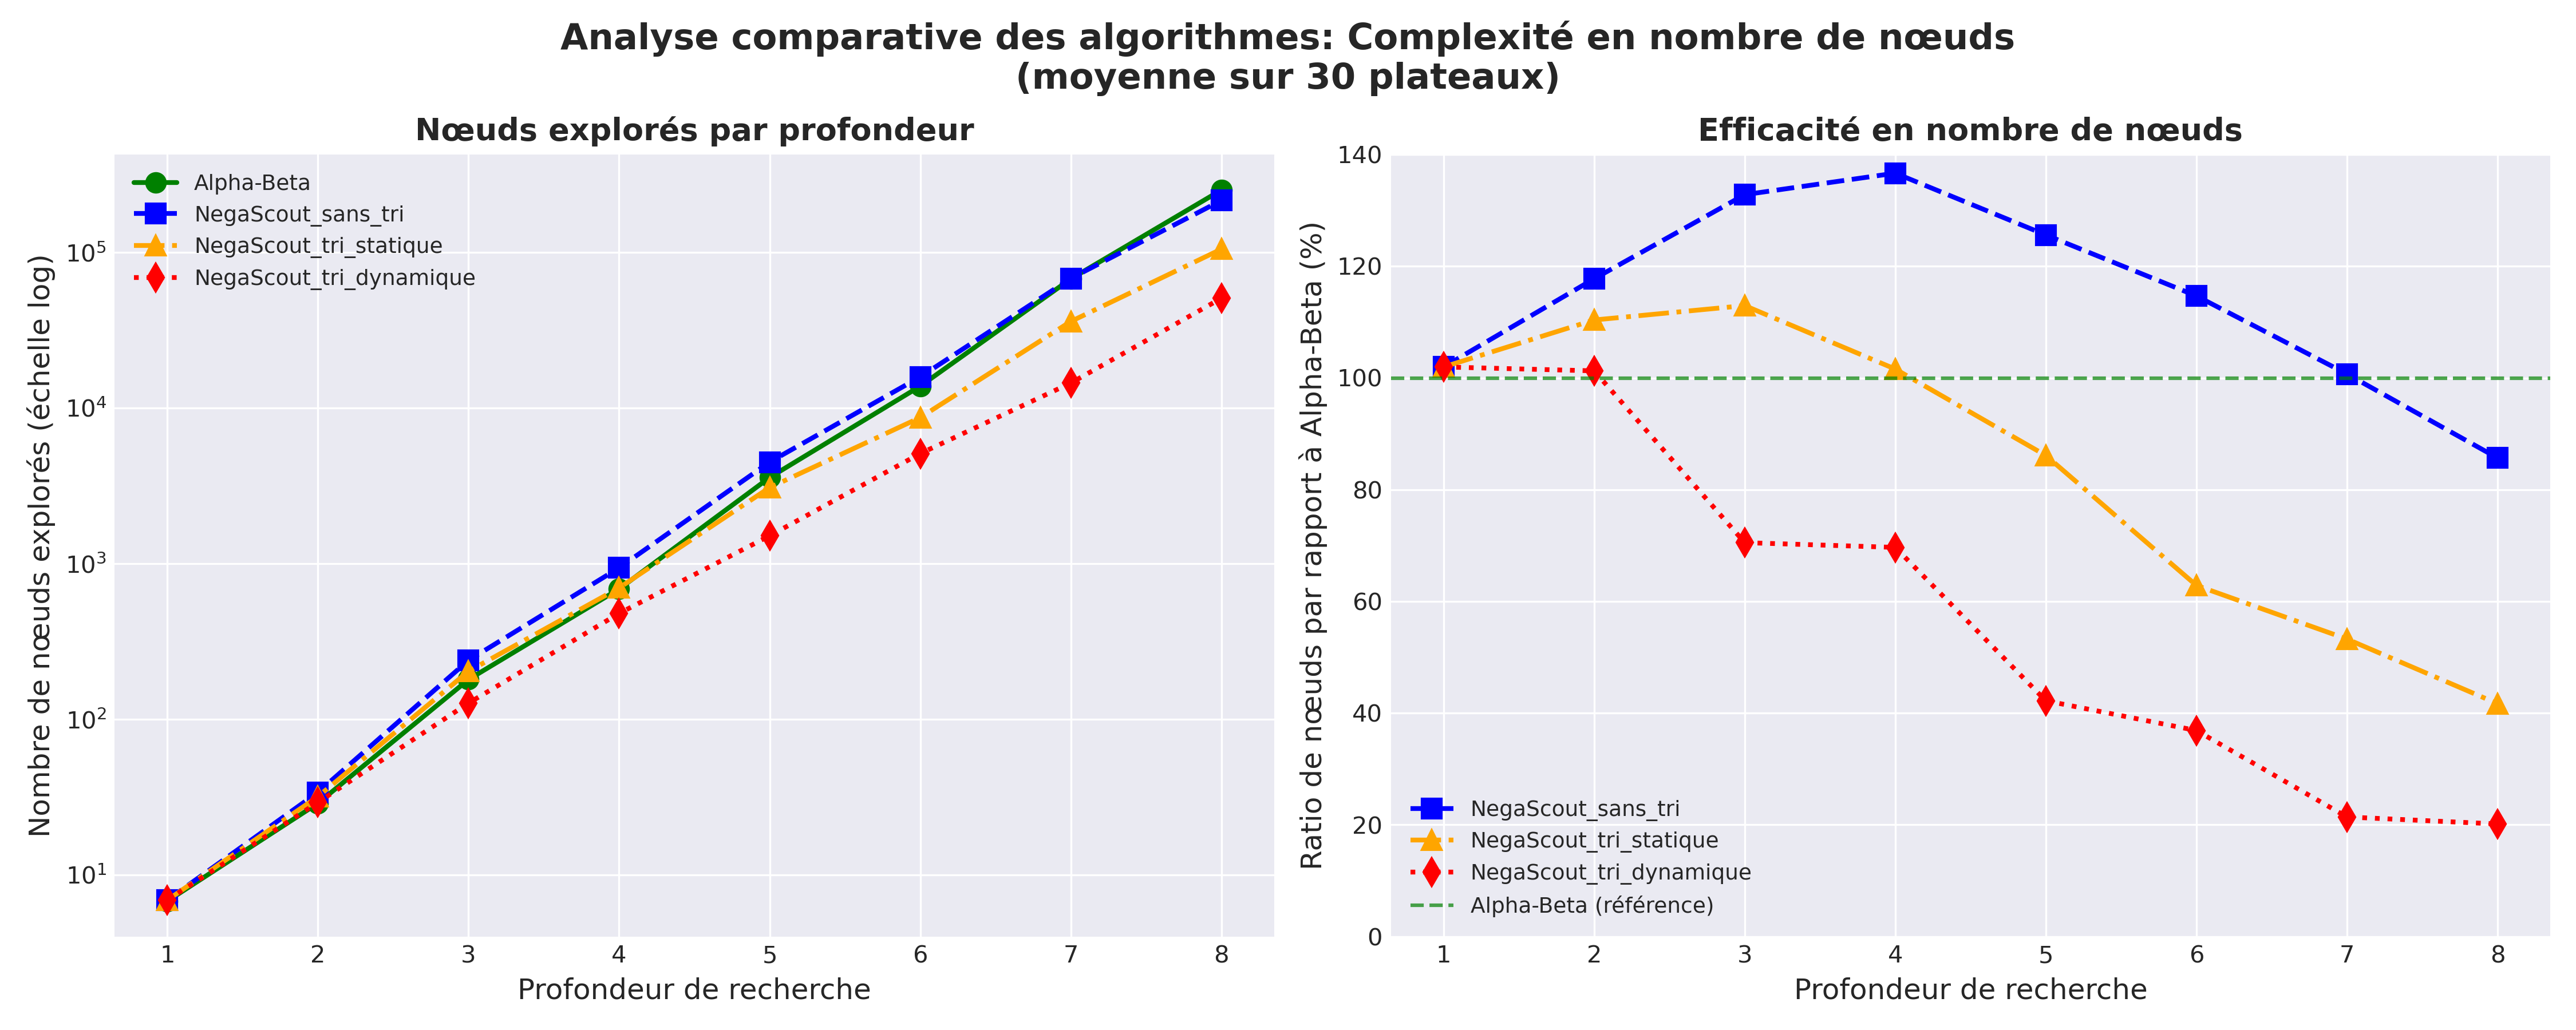
\includegraphics[width=\textwidth]{../assets/analyse_noeuds.png}
            \scriptsize{Analyse du nombre de nœuds explorés}
            
            \begin{itemize}\scriptsize
                \item \textbf{Tri dynamique} : plus efficace (jusqu'à 80\% de réduction)
                \item \textbf{Tri statique} : bon compromis (40-60\% de réduction à grande profondeur)
                \item \textbf{NegaScout sans tri} : inefficace à faible profondeur, mais s'améliore
            \end{itemize}
        \end{column}
        \begin{column}{0.48\textwidth}
            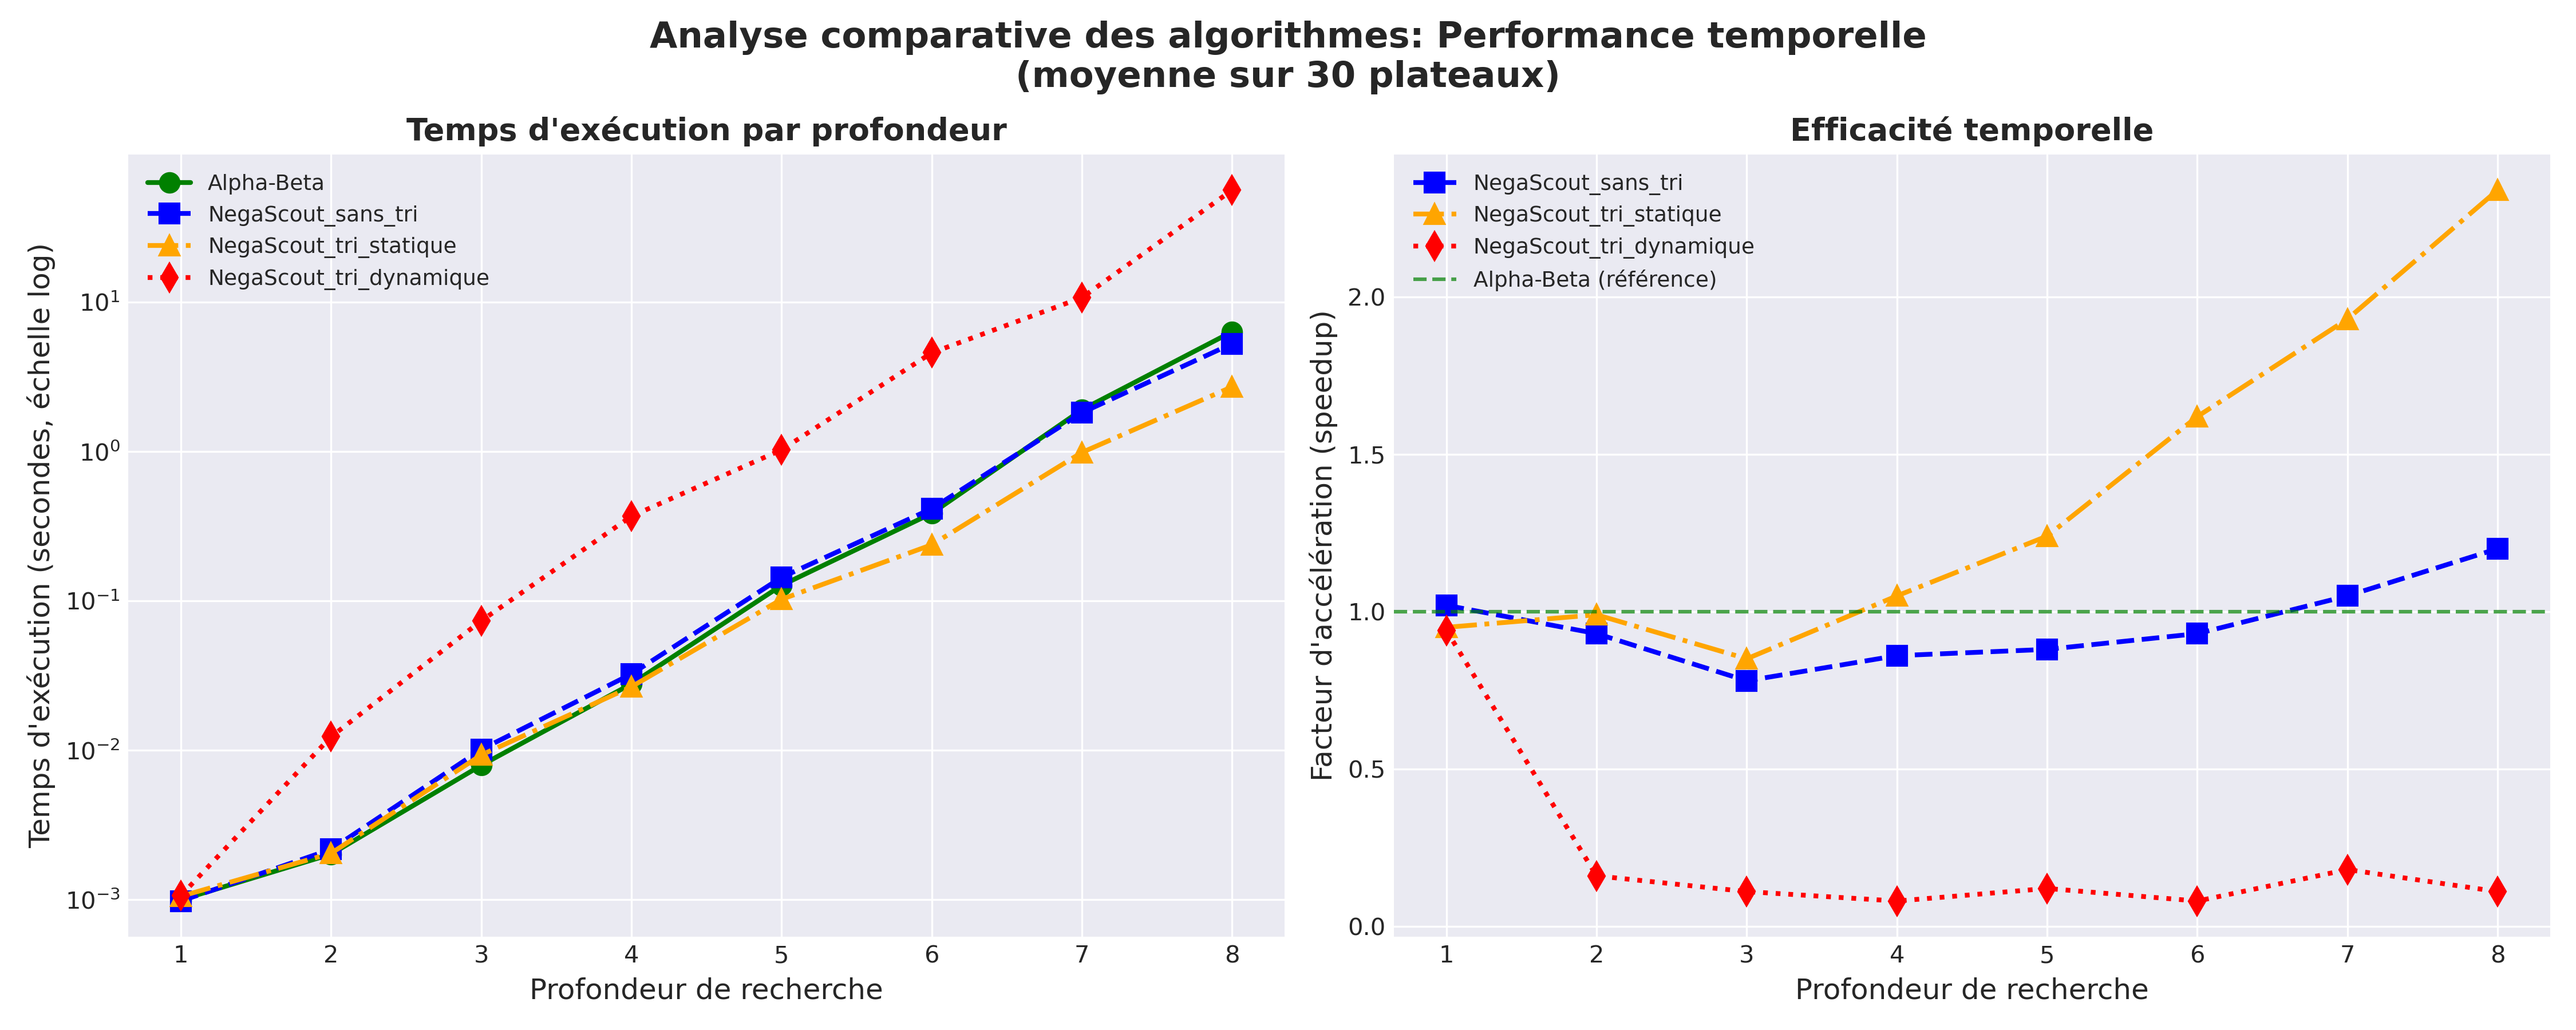
\includegraphics[width=\textwidth]{../assets/analyse_temps.png}
            \scriptsize{Analyse du temps d'exécution}
            
            \begin{itemize}\scriptsize
                \item \textbf{Tri statique} : nettement plus rapide (jusqu'à 2,3× d'accélération)
                \item \textbf{Tri dynamique} : malgré moins de nœuds, trop coûteux en temps
                \item \textbf{NegaScout sans tri} : performances comparables à Alpha-Beta
            \end{itemize}
        \end{column}
    \end{columns}
    
    \begin{block}{Conclusion}
    \scriptsize
    \begin{itemize}
        \item Le tri statique offre le meilleur compromis performance/temps et a été retenu
        \item À grande profondeur, il réduit de 60\% les nœuds explorés et accélère de 230\% le temps
    \end{itemize}
    \end{block}
\end{frame}

\section{Endgame et évaluation avancée}

\begin{frame}
    \frametitle{Détection d'endgame et évaluation adaptative}
    
    \begin{columns}
        \begin{column}{0.48\textwidth}
            \begin{block}{Détection de l'endgame}
            \scriptsize
            \begin{itemize}
                \item Critères précis : cases vides $\leq 14$, mobilité $\leq 8$, coins $\geq 3$
                \item Augmentation auto. de profondeur (+6)
                \item Recherche exhaustive pour score optimal
            \end{itemize}
            \end{block}
            
            \begin{block}{Critères stratégiques}
            \scriptsize
            \begin{itemize}
                \item \textbf{Mobilité} : coups légaux, frontière
                \item \textbf{Stabilité} : pions inretournables
                \item \textbf{Parité} : avantage cases vides pair/impair
                \item \textbf{Disk-Square Tables} : valeurs positionnelles
            \end{itemize}
            \end{block}
        \end{column}
        
        \begin{column}{0.48\textwidth}
            \begin{block}{Pondération par phase}
            \scriptsize
            \begin{itemize}
                \item \textbf{Début} : mobilité (×5), positions (×2)
                \item \textbf{Milieu} : mobilité (×4), stabilité (×3), ensembles (×3)
                \item \textbf{Fin} : stabilité (×6), parité (×3)
            \end{itemize}
            \end{block}
        \end{column}
    \end{columns}
\end{frame}

\section{Conclusion}

\begin{frame}
    \frametitle{Conclusion et résultats obtenus}
    
    \begin{block}{Améliorations quantifiables}
    \scriptsize
    \begin{itemize}
        \item \textbf{Mémoire} : réduction de 98\% à profondeur 3, jusqu'à 99,99\% à profondeur 7
        \item \textbf{Performance} : NegaScout avec tri statique explore 60\% moins de nœuds et accélère le temps de 230\%
        \item \textbf{Endgame} : détection précise permettant d'augmenter la profondeur de 6 niveaux
    \end{itemize}
    \end{block}
    
    \begin{block}{Compétences développées}
    \scriptsize
    \begin{itemize}
        \item Optimisation algorithmique et gestion fine de la mémoire
        \item Analyse comparative et prise de décision basée sur les données
        \item Implémentation d'heuristiques avancées pour l'IA de jeux
        \item Développement incrémental avec validation expérimentale
    \end{itemize}
    \end{block}
    
    \begin{center}
        \large\textbf{Merci de votre attention}
    \end{center}
\end{frame}

\end{document}